% ============================================================
% CAPITOLO 6 — Il backtest
% Scritto il 2026-09-13 seguendo il programma in frontmatter/abstract.tex.
% Copre scripts/06_run_backtest.py e src/cryptognn/evaluation/backtest.py.
% Assorbe YYY_literature-review.tex (sec:evaluation-metrics-methodological-
% pitfalls, "Scelta della metrica di valutazione") e ZZZ_old-case-study.tex
% ("Il costo economico"). Decisioni di sessione:
%   - Label con prefisso bt- e tabella ricopiata inline (non
%     \begin{table}[H]
\centering
\caption[Metriche economiche della strategia sul segno]{Strategia sul segno della previsione, equipesata sui 15 asset e ribilanciata ogni giorno, sui $1\,512$ giorni del periodo di test. Ogni misura è riportata a 0 e a 10 punti base di costo, applicati a ogni cambio di posizione; lo Sharpe è annualizzato su 365 giorni e non sottrae un tasso privo di rischio. Il buy-and-hold è il paniere equipesato acquistato il primo giorno e mantenuto, e non usa alcuna previsione: serve da termine di paragone. La previsione nulla non prende posizione, quindi il suo Sharpe non è definito.}
\label{tab:backtest}
\small
\begin{tabular}{@{}lrrrrrr@{}}
\toprule
 & \multicolumn{2}{c}{\textbf{Sharpe}} & \multicolumn{2}{c}{\textbf{Max drawdown}} & \multicolumn{2}{c}{\textbf{Rend. cumulato}} \\
\cmidrule(lr){2-3}\cmidrule(lr){4-5}\cmidrule(lr){6-7}
\textbf{Modello} & \textbf{0 bps} & \textbf{10 bps} & \textbf{0 bps} & \textbf{10 bps} & \textbf{0 bps} & \textbf{10 bps} \\
\midrule
Zero & -- & -- & $0{,}0\%$ & $0{,}0\%$ & $0{,}0\%$ & $0{,}0\%$ \\
Media storica & $-0{,}665$ & $-0{,}671$ & $-84{,}4\%$ & $-84{,}5\%$ & $-80{,}5\%$ & $-80{,}7\%$ \\
AR & $-0{,}596$ & $-0{,}718$ & $-79{,}1\%$ & $-82{,}9\%$ & $-75{,}6\%$ & $-80{,}3\%$ \\
VAR (BIC) & $-0{,}665$ & $-0{,}671$ & $-84{,}4\%$ & $-84{,}5\%$ & $-80{,}5\%$ & $-80{,}7\%$ \\
VAR ($p=5$) & $0{,}147$ & $-0{,}612$ & $-60{,}6\%$ & $-87{,}0\%$ & $-16{,}2\%$ & $-81{,}2\%$ \\
GCN & $0{,}453$ & $0{,}014$ & $-66{,}0\%$ & $-83{,}8\%$ & $43{,}1\%$ & $-55{,}1\%$ \\
GCN senza grafo & $0{,}610$ & $0{,}051$ & $-44{,}2\%$ & $-59{,}3\%$ & $108{,}2\%$ & $-31{,}5\%$ \\
Buy-and-hold & $0{,}262$ & $0{,}261$ & $-66{,}9\%$ & $-66{,}9\%$ & $-14{,}7\%$ & $-14{,}8\%$ \\
\bottomrule
\end{tabular}
\end{table}
) perché ZZZ, ancora \input, definisce già
%     tab:backtest e fig:equity-curves.
%   - Alla tabella generata è aggiunta la colonna del turnover medio, presa
%     da project-thesis/results/summary.md: la lettura dei risultati si regge
%     su quella colonna.
%   - report() di 06_run_backtest.py è descritto in prosa, senza snippet.
%   - Nei blocchi minted le omissioni rispetto al sorgente sono segnate da
%     "# ..."; per il resto il codice è verbatim.
% ============================================================
\chapter{Il backtest}
\label{ch:backtest}

Il \Cref{ch:training-and-comparison} si è chiuso con un esito negativo: nessuno dei sei modelli batte la baseline \texttt{ZeroForecaster} in errore quadratico, e la GCN non si distingue dalla propria ablation. Questo verdetto riguarda però l'accuratezza, e non consente di trarre conclusioni sul valore delle previsioni per chi le usa. I due risultati non devono necessariamente coincidere: l'errore quadratico è dominato dalle giornate in cui una previsione sbaglia maggiormente, mentre una strategia che opera sul suo segno tiene conto solamente della direzione. Un modello può quindi avere l'RMSE peggiore, ma la strategia migliore. Questo capitolo misura il valore economico delle previsioni seguendo lo script \path{06_run_backtest.py}.

\section{Oltre l'errore di previsione}
\label{sec:bt-beyond-accuracy}

L'RMSE e il MAE sono metriche standard per la regressione, poco informative però sui rendimenti finanziari. Il motivo discende direttamente dagli \emph{stylized facts} della \cref{sec:stylized-facts}: i rendimenti hanno media prossima a zero e un'autocorrelazione lineare di intensità contenuta, quindi il predittore costante $\hat r=0$ ottiene già un RMSE vicino a quello ottimo. Sul periodo di test dello studio vale $0{,}04145$ (\cref{tab:tc-results-main}). Un modello può ridurre questo valore di una frazione di punto percentuale senza che il miglioramento si distingua dal rumore. Un RMSE eccellente, inoltre, è compatibile con un modello che sbaglia sistematicamente il segno.

L'accuratezza direzionale misura ciò che serve per applicare il modello ai casi reali, ma tratta allo stesso modo un movimento dello $0{,}1\%$ e uno del $20\%$. Un modello può quindi predire correttamente il segno nel $60\%$ dei casi e perdere comunque denaro se sbaglia proprio nelle giornate che contano.

Le metriche economiche rispondono direttamente alla domanda rilevante per un investitore, ovvero se le previsioni producano un profitto al netto dei costi. Si costruisce una strategia che opera sulle previsioni e se ne misurano il rendimento cumulato, il rendimento in rapporto alla volatilità e la perdita peggiore subita. Queste metriche dipendono però da ipotesi come quella sui costi di transazione, dichiarata esplicitamente dalla pipeline.

\section{Le misure di performance}
\label{sec:bt-metrics}

\subsection{Sharpe ratio}
\label{sec:bt-sharpe}

Sia $x_1,\dots,x_n$ la serie dei rendimenti giornalieri di una strategia. Lo Sharpe ratio~\cite{sharpe1966mutual,sharpe1994sharpe} adottato dallo studio rapporta il rendimento medio alla sua variabilità,
\begin{equation}
\label{eq:bt-sharpe}
\mathrm{SR}=\sqrt{P}\,\frac{\bar x}{s},\qquad \bar x=\frac1n\sum_{t=1}^n x_t,\qquad s^2=\frac{1}{n-1}\sum_{t=1}^n(x_t-\bar x)^2,
\end{equation}
dove $P$ è il numero di periodi in un anno. Il fattore $\sqrt{P}$ annualizza il rapporto. La media cresce infatti linearmente con l'orizzonte e la deviazione standard con la sua radice, se i rendimenti sono indipendenti. Lo Sharpe ratio quantifica il rendimento medio per unità di rischio, dove il rischio è identificato con la deviazione standard dei rendimenti. Non misura quindi la redditività assoluta della strategia, ma la sua efficienza nell'impiego della volatilità sostenuta. A parità di $\bar x$, un incremento della dispersione $s$ riduce proporzionalmente l'indicatore, penalizzando le strategie il cui rendimento deriva da oscillazioni di ampiezza elevata.

\begin{listing}[H]
\begin{minted}{python}
def sharpe(returns: np.ndarray, periods: int = PERIODS_PER_YEAR) -> float:
    returns = np.asarray(returns, dtype=float)
    # Check the series is one-dimensional and the periods per year are positive.
    ...
    if returns.size < 2:
        return float("nan")

    deviation = float(returns.std(ddof=1))
    if deviation == 0.0:
        return float("nan")
    return float(returns.mean() / deviation * np.sqrt(periods))
\end{minted}
\caption{\texttt{sharpe}}
\label{lst:sharpe}
\end{listing}

Nella definizione originale~\cite{sharpe1966mutual}, il numeratore corrisponde al rendimento in eccesso della strategia rispetto ad un'attività priva di rischio: detto $r_{f,t}$ il rendimento di quest'ultima nel periodo $t$ e posto $x_{e,t}=x_t-r_{f,t}$, lo Sharpe ratio è
\[
\mathrm{SR}_e=\sqrt{P}\,\frac{\bar x_e}{s_e},\qquad
\bar x_e=\frac1n\sum_{t=1}^n x_{e,t},\qquad
s_e^2=\frac{1}{n-1}\sum_{t=1}^n(x_{e,t}-\bar x_e)^2.
\]
L'equazione~\eqref{eq:bt-sharpe}, che la funzione implementa, ne è il caso particolare $r_{f,t}=0$ per ogni $t$. La pipeline adotta tale variante perché, tra il 2022 e il 2026, il tasso a breve è passato da valori prossimi a zero a circa il $5\%$; pertanto un valore unico sarebbe sbagliato per gran parte del campione.

La costante \texttt{PERIODS\_PER\_YEAR} vale $365$ e non $252$. Come accennato nella \cref{sec:stylized-facts}, il mercato delle criptovalute non è soggetto ad interruzioni o pause e non ci sono giornate da escludere. Usare $252$ ridurrebbe tutti gli Sharpe ratio di un fattore $\sqrt{252/365}\approx0{,}83$.

Una serie costante, inoltre, ha deviazione standard nulla e l'equazione~\eqref{eq:bt-sharpe} non è definita. La funzione restituisce allora \texttt{NaN}, allineandosi al caso della previsione nulla che non prende mai posizione e ha tutti i rendimenti giornalieri nulli. Uno Sharpe pari a $0$ si leggerebbe come una strategia dal rendimento piatto, quando invece la strategia non esiste. La convenzione è la stessa già adottata dall'accuratezza direzionale nella \cref{sec:tc-skill-score}.

\subsection{Massimo drawdown}
\label{sec:bt-drawdown}

Sia $E_0,\dots,E_n$ la curva del capitale, ottenuta reinvestendo integralmente il risultato di ogni periodo: posto $E_0=1$, il capitale evolve secondo la ricorsione $E_t=E_{t-1}(1+x_t)$, cosicché $E_t$ è il valore di un investimento unitario iniziale dopo $t$ periodi. Esplicitando la ricorsione si ottiene la forma moltiplicativa
\[
E_t=\prod_{i=1}^{t}(1+x_i),\qquad t=0,\dots,n,
\]
con la convenzione che il prodotto vuoto valga $1$. La composizione è moltiplicativa, motivo per cui una perdita e un guadagno di pari entità percentuale non si compensano.

Si definisce drawdown all'istante $t$ lo scostamento relativo del capitale dal massimo raggiunto fino a quell'istante, $D_t=\dfrac{E_t}{\max_{0\leq s\leq t}E_s}-1$. Il massimo drawdown è il minimo corrente di tale successione,
\begin{equation}
\label{eq:bt-max-drawdown}
\mathrm{MDD}=\min_{0\leq t\leq n}D_t=\min_{0\leq t\leq n}\left(\frac{\max(E_t,0)}{\max_{0\leq s\leq t}E_s}-1\right).
\end{equation}
È un numero compreso tra $-1$ e $0$: vale $0$ per una curva che non scende mai sotto il proprio massimo precedente e tende a $-1$ quando il capitale viene eroso quasi per intero. Misura la peggiore perdita che un investitore avrebbe sperimentato entrando nel momento meno favorevole, ovvero l'ampiezza massima della fase di ritracciamento subita dalla strategia sull'intero periodo.

\begin{listing}[H]
\begin{minted}{python}
def max_drawdown(equity: np.ndarray) -> float:
    equity = np.asarray(equity, dtype=float)
    # Check the curve is one-dimensional and return NaN if it is empty.
    ...
    peak = np.maximum.accumulate(equity)
    if peak[0] <= 0:
        raise ValueError(f"Equity curve starts at {equity[0]}: a drawdown needs positive capital to fall from")
    return float(np.min(np.maximum(equity, 0.0) / peak - 1.0))
\end{minted}
\caption{\texttt{max\_drawdown}}
\label{lst:max-drawdown}
\end{listing}

Il massimo cumulato \texttt{np.maximum.accumulate} calcola il picco $\max_{s\leq t}E_s$ per ogni $t$ in un solo passaggio. Il picco parte dal primo elemento della serie ricevuta: se la curva cominciasse da $E_1$ anziché da $E_0$, il picco iniziale coinciderebbe con $E_1$ e la caduta da $E_0$ a $E_1$ non verrebbe mai contata. Per questo, la funzione che riassume una strategia antepone il capitale iniziale $E_0=1$, con \texttt{np.concatenate(([1.0], equity))}. Il termine \texttt{np.maximum(equity, 0.0)} realizza il pavimento a $-1$ dell'equazione~\eqref{eq:bt-max-drawdown}. Una strategia che vende allo scoperto può in linea di principio perdere più del proprio capitale. Oltre la perdita totale non resta però nulla da perdere e un drawdown di $-1{,}4$ non avrebbe significato.

\section{La strategia sul segno}
\label{sec:bt-strategy}

Per trasformare le previsioni in rendimenti è necessaria una strategia. Sia $\hat r_{t,i}$ la previsione del log-rendimento dell'asset $i$ realizzato nel giorno $t$. Quella adottata dal progetto assume ogni giorno su ciascuno degli $N=15$ asset una posizione lunga (\emph{long}) se la previsione è positiva e corta (\emph{short}) se è negativa, con peso
\begin{equation}
\label{eq:bt-weights}
w_{t,i}=\frac{\operatorname{sign}(\hat r_{t,i})}{N}.
\end{equation}
Il portafoglio è equipesato e ribilanciato ogni giorno. Non interviene alcuna ottimizzazione: non si dimensionano le posizioni in base alla fiducia nella previsione, non si controlla la volatilità e non si scelgono gli asset su cui operare.

Il denominatore è $N$ fisso e non il numero di posizioni diverse da zero. L'esposizione lorda $\sum_i|w_{t,i}|$ resta in questo modo al più $1$ e le curve dei diversi modelli sono confrontabili. Normalizzare per il numero di posizioni attive aumenterebbe la leva di un modello proprio nei giorni in cui è indeciso.

Le posizioni sono applicate ai rendimenti semplici, non ai log-rendimenti. La \cref{sec:returns-stationarity} ha mostrato che le due grandezze coincidono solo per variazioni piccole. Una posizione corta non guadagna $-r_{t,i}$ ma $-R_{t,i}=-(e^{r_{t,i}}-1)$. Sulla giornata da $-30\%$ del \cref{ch:dynamic-correlation-graph}, con $r=-0{,}357$, una posizione corta guadagna il $30\%$ e non il $35{,}7\%$. Il rendimento lordo della strategia è quindi
\begin{equation}
\label{eq:bt-gross-return}
x_t^{\mathrm{lordo}}=\sum_{i=1}^N w_{t,i}\,R_{t,i},\qquad R_{t,i}=e^{r_{t,i}}-1.
\end{equation}

L'equazione~\eqref{eq:bt-weights} è implementata da \texttt{sign\_strategy} (\cref{lst:sign-strategy}), che riceve la tabella delle previsioni prodotta da \texttt{run\_walkforward} (\cref{sec:tc-walkforward}), con una riga per data, asset e modello.

\begin{listing}[H]
\begin{minted}{python}
def sign_strategy(predictions: pd.DataFrame, cost_bps: float) -> pd.DataFrame:
    forecast = _panel(predictions, "y_pred")
    realized = np.expm1(_panel(predictions, "y_true"))
    return _curve(np.sign(forecast) / forecast.shape[1], realized, cost_bps)
\end{minted}
\caption{\texttt{sign\_strategy}}
\label{lst:sign-strategy}
\end{listing}

La funzione ausiliaria \texttt{\_panel} converte il DataFrame \texttt{predictions} in una matrice di $\mathbb{R}^{n\times N}$, con una riga per data e una colonna per asset, e solleva un errore se manca anche solo una cella. Un valore mancante produrrebbe un rendimento \texttt{NaN} che, propagato nel prodotto cumulato, svuoterebbe l'intera curva da quel giorno in poi. I rendimenti semplici sono ottenuti con \texttt{np.expm1}, che calcola $e^r-1$ senza perdita di precisione per $r$ piccolo. Il costo non è direttamente utilizzato da \texttt{sign\_strategy}, che si occupa di inoltrarlo alla funzione \texttt{\_curve} (\cref{lst:curve}), la quale lo addebita secondo la \cref{sec:bt-cost}.

Il rendimento realizzato, inoltre, non è passato come argomento separato. La tabella contiene già \texttt{y\_true} e \texttt{y\_pred} sulla stessa riga e una seconda fonte potrebbe introdurre un disallineamento, errore che non produrrebbe un'eccezione ma renderebbe la curva plausibile e sbagliata.

\section{Il riferimento buy-and-hold}
\label{sec:bt-benchmark}

Le misure di una singola strategia non sono interpretabili in assoluto, ma solo rispetto al mercato sugli stessi giorni. Serve quindi un termine di paragone che non usi alcuna previsione, costruito da \texttt{buy\_and\_hold} (\cref{lst:buy-and-hold}).

\begin{listing}[H]
\begin{minted}{python}
def buy_and_hold(predictions: pd.DataFrame, cost_bps: float) -> pd.DataFrame:
    realized = np.expm1(_panel(predictions.drop_duplicates(["date", "asset"]), "y_true"))
    positions = pd.DataFrame(1.0 / realized.shape[1], index=realized.index, columns=realized.columns)
    return _curve(positions, realized, cost_bps)
\end{minted}
\caption{\texttt{buy\_and\_hold}}
\label{lst:buy-and-hold}
\end{listing}

Il buy-and-hold assume una posizione lunga di peso $1/N$ su ogni asset per l'intero periodo. È l'unica strategia della tabella che non usa alcuna previsione. Poiché i pesi non cambiano mai, il suo turnover è $1$ il primo giorno e $0$ in tutti gli altri.

\section{Costi e curva del capitale}
\label{sec:bt-costs-and-curve}

\subsection{Il costo di transazione}
\label{sec:bt-cost}

Ogni cambio di posizione ha un costo, dovuto alle commissioni applicate dall'exchange, al differenziale tra denaro e lettera (\emph{bid-ask spread}) e allo scostamento tra il prezzo atteso e quello di effettiva esecuzione (\emph{slippage}). Il turnover del giorno $t$ misura quanto il portafoglio è cambiato rispetto al giorno precedente,
\begin{equation}
\label{eq:bt-turnover}
u_t=\sum_{i=1}^N\left|w_{t,i}-w_{t-1,i}\right|,\qquad w_{0,i}=0.
\end{equation}
Il portafoglio parte vuoto, quindi il primo giorno paga l'ingresso come qualunque altro cambio di posizione. Il costo è proporzionale al turnover secondo un'aliquota $c$ espressa in \emph{basis point}, ovvero in centesimi di punto percentuale. È l'unità in cui le borse pubblicano le proprie commissioni. Il rendimento netto e il capitale sono
\begin{equation}
\label{eq:bt-net-return}
x_t=x_t^{\mathrm{lordo}}-c\cdot10^{-4}\,u_t,\qquad E_t=\prod_{s=1}^t(1+x_s).
\end{equation}
Un modello che inverte il segno di tutte le previsioni da un giorno all'altro ha $u_t=2$ e paga $2c$ basis point. Un modello che non cambia mai posizione paga solo l'ingresso. Il turnover è calcolato sui pesi e non tiene conto della deriva delle posizioni dovuta ai rendimenti del giorno. Il ribilanciamento verso pesi uguali non viene quindi addebitato, una semplificazione che vale allo stesso modo per tutte le strategie.

\subsection{Dalle posizioni al capitale}
\label{sec:bt-curve}

La strategia sul segno e il buy-and-hold passano dalla stessa funzione \texttt{\_curve}, che implementa le equazioni~\eqref{eq:bt-gross-return}, \eqref{eq:bt-turnover} e~\eqref{eq:bt-net-return}.

\begin{listing}[H]
\begin{minted}{python}
def _curve(positions: pd.DataFrame, simple_returns: pd.DataFrame, cost_bps: float) -> pd.DataFrame:
    if cost_bps < 0:
        raise ValueError(f"Transaction cost must be non-negative, got {cost_bps} bps")

    gross = (positions * simple_returns).sum(axis=1)
    turnover = (positions - positions.shift(1).fillna(0.0)).abs().sum(axis=1)
    cost = turnover * cost_bps * BASIS_POINT
    net = gross - cost

    return pd.DataFrame(
        {
            "date": positions.index,
            "gross_return": gross.to_numpy(),
            "turnover": turnover.to_numpy(),
            "cost": cost.to_numpy(),
            "net_return": net.to_numpy(),
            "equity": (1.0 + net).cumprod().to_numpy(),
        }
    )
\end{minted}
\caption{\texttt{\_curve}}
\label{lst:curve}
\end{listing}

Il prodotto \texttt{positions * simple\_returns} è elemento per elemento e la somma per riga restituisce $x_t^{\mathrm{lordo}}$. L'istruzione \texttt{positions.shift(1).fillna(0.0)} costruisce $w_{t-1,i}$, con il valore nullo del primo giorno, che corrisponde a $w_{0,i}=0$. La costante \texttt{BASIS\_POINT} vale $10^{-4}$ ed è utilizzata per convertire \texttt{cost\_bps} da basis point a frazione del capitale. Il capitale è il prodotto cumulato di $1+x_t$. La posizione non viene chiusa l'ultimo giorno, perché liquidare alla fine del campione non è una decisione della strategia. Condividere \texttt{\_curve} tra le due strategie garantisce che la contabilità dei costi sia identica per il modello misurato e per il suo termine di paragone.

\section{Risultati}
\label{sec:bt-results}

La \Cref{tab:bt-backtest} riporta le misure delle otto strategie valutate — i sette modelli del \cref{ch:training-and-comparison}, ciascuno attraverso la strategia sul segno, e il buy-and-hold — sui $1512$ giorni del periodo di test, dal 05/05/2022 al 24/06/2026, ai due livelli di costo. Le previsioni non sono ricalcolate in questa fase, ma sono quelle fissate dagli addestramenti del \cref{ch:training-and-comparison} e rilette dal disco.

Il livello di costo positivo, che vale $10$ basis point nella pipeline di progetto, e quello nullo sono valutati nella stessa esecuzione. La distanza tra gli Sharpe a costi diversi, che corrisponde all'informazione da ricavare, è più affidabile se le sue parti provengono dallo stesso codice applicato agli stessi giorni.

\begin{table}[H]
\centering
\caption[Metriche economiche della strategia sul segno]{Strategia sul segno della previsione, equipesata sui $15$ asset e ribilanciata ogni giorno, sui $1\,512$ giorni del periodo di test, a $0$ e a $10$ basis point di costo. Lo Sharpe è annualizzato su $365$ giorni e non sottrae un tasso privo di rischio. Il turnover è la media giornaliera e non dipende dal costo. Il buy-and-hold non usa alcuna previsione e serve da termine di paragone. La previsione nulla non prende posizione, quindi il suo Sharpe non è definito.}
\label{tab:bt-backtest}
\small
\setlength{\tabcolsep}{4pt}
\begin{tabular}{@{}lrrrrrrr@{}}
\toprule
 & \multicolumn{2}{c}{\textbf{Sharpe}} & \multicolumn{2}{c}{\textbf{Max drawdown}} & \multicolumn{2}{c}{\textbf{Rend. cumulato}} & \\
\cmidrule(lr){2-3}\cmidrule(lr){4-5}\cmidrule(lr){6-7}
\textbf{Modello} & \textbf{0 bps} & \textbf{10 bps} & \textbf{0 bps} & \textbf{10 bps} & \textbf{0 bps} & \textbf{10 bps} & \textbf{Turnover} \\
\midrule
Zero & -- & -- & $0{,}0\%$ & $0{,}0\%$ & $0{,}0\%$ & $0{,}0\%$ & $0{,}000$ \\
Media storica & $-0{,}665$ & $-0{,}671$ & $-84{,}4\%$ & $-84{,}5\%$ & $-80{,}5\%$ & $-80{,}7\%$ & $0{,}007$ \\
AR & $-0{,}596$ & $-0{,}718$ & $-79{,}1\%$ & $-82{,}9\%$ & $-75{,}6\%$ & $-80{,}3\%$ & $0{,}141$ \\
VAR (BIC) & $-0{,}665$ & $-0{,}671$ & $-84{,}4\%$ & $-84{,}5\%$ & $-80{,}5\%$ & $-80{,}7\%$ & $0{,}007$ \\
VAR ($p=5$) & $0{,}147$ & $-0{,}612$ & $-60{,}6\%$ & $-87{,}0\%$ & $-16{,}2\%$ & $-81{,}2\%$ & $0{,}987$ \\
GCN & $0{,}453$ & $0{,}014$ & $-66{,}0\%$ & $-83{,}8\%$ & $43{,}1\%$ & $-55{,}1\%$ & $0{,}766$ \\
GCN senza grafo & $0{,}610$ & $0{,}051$ & $-44{,}2\%$ & $-59{,}3\%$ & $108{,}2\%$ & $-31{,}5\%$ & $0{,}735$ \\
Buy-and-hold & $0{,}262$ & $0{,}261$ & $-66{,}9\%$ & $-66{,}9\%$ & $-14{,}7\%$ & $-14{,}8\%$ & $0{,}001$ \\
\bottomrule
\end{tabular}
\end{table}

\subsection{Senza costi di transazione}

Senza costi di transazione, la GCN e la sua ablation ottengono gli Sharpe ratio più alti della tabella, rispettivamente $0{,}453$ e $0{,}610$, superando il buy-and-hold ($0{,}262$). Il rendimento è del $43{,}1\%$ per la GCN e del $108{,}2\%$ per la variante senza grafo, a fronte del $-14{,}7\%$ del portafoglio di riferimento. La variante senza grafo ha anche il drawdown meno profondo, $-44{,}2\%$ contro il $-66{,}0\%$ della GCN. Il VAR con ordine fissato ha uno Sharpe appena positivo ($0{,}147$). Le altre baseline perdono in modo consistente.

Il risultato non contraddice il \cref{ch:training-and-comparison}. La GCN ha lo skill score peggiore tra i due bracci e un'accuratezza direzionale del $50{,}9\%$, ma la strategia sul segno è insensibile all'ampiezza degli errori: conta solo che le giornate in cui il segno è corretto coincidano con movimenti ampi.

La media storica e il VAR selezionato per BIC producono righe identiche, perché coincidono numericamente (\cref{sec:var-baseline}). La loro previsione è costante all'interno di ciascun fold, quindi le posizioni cambiano solo al passaggio da un fold al successivo e il turnover medio è di appena $0{,}007$. La previsione nulla non prende mai posizione: il suo capitale resta pari a $1$ e lo Sharpe non è definito.

Il buy-and-hold mostra che le misure della tabella non vanno lette isolatamente: il suo Sharpe è positivo mentre il rendimento cumulato è negativo. Lo Sharpe usa la media aritmetica dei rendimenti giornalieri, mentre il capitale li compone in modo geometrico. Con una volatilità elevata come quella delle criptovalute la differenza tra le due medie è ampia. Una sequenza di $+50\%$ e $-50\%$ ha media aritmetica nulla ma riduce il capitale a $0{,}75$.

\subsection{Con i costi di transazione}

\begin{figure}[H]
\centering
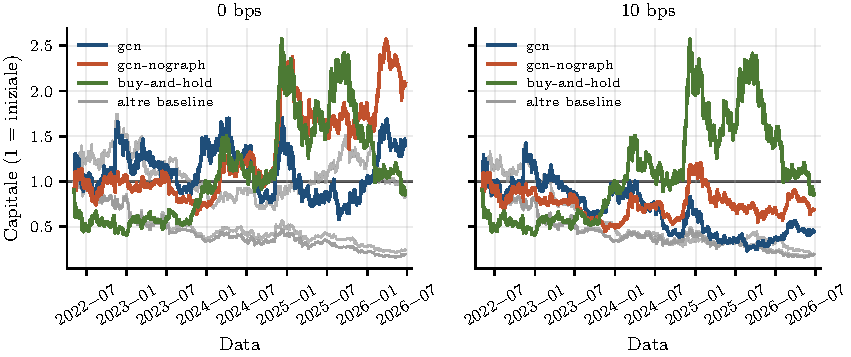
\includegraphics[width=\textwidth]{figures/fig_equity_curves.pdf}
\caption[Curve del capitale della strategia sul segno]{Capitale della strategia sul segno nel periodo di test, a $0$ e a $10$ basis point di costo, sullo stesso asse verticale. Sono evidenziati i due bracci della GCN e il buy-and-hold. Le altre baseline sono in grigio.}
\label{fig:bt-equity-curves}
\end{figure}

A $10$ basis point la classifica si inverte. Lo Sharpe della GCN scende da $0{,}453$ a $0{,}014$ e quello della variante senza grafo da $0{,}610$ a $0{,}051$. Il buy-and-hold resta pressoché invariato a $0{,}261$. Il rendimento cumulato dei due bracci diventa negativo, $-55{,}1\%$ e $-31{,}5\%$. La \Cref{fig:bt-equity-curves} mostra la stessa erosione nel tempo: a costo zero le curve dei due bracci terminano sopra il capitale iniziale; con i costi scivolano entrambe sotto di esso, mentre la curva del portafoglio di riferimento è la stessa nei due pannelli.

La colonna del turnover spiega il ribaltamento. Le reti cambiano posizione quasi ogni giorno, con un turnover medio di $0{,}766$ per la GCN e $0{,}735$ per la variante senza grafo. Per l'equazione~\eqref{eq:bt-net-return} questo costa in media circa $7{,}5$ basis point al giorno, cioè oltre il $27\%$ del capitale all'anno prima di ogni composizione. Il VAR con ordine fissato ha il turnover più alto, $0{,}987$. Il suo Sharpe passa da $0{,}147$ a $-0{,}612$. All'estremo opposto il buy-and-hold paga solo l'ingresso ($0{,}001$) e la media storica solo i cambi di fold ($0{,}007$). L'AR, con un turnover intermedio di $0{,}141$, perde $0{,}12$ di Sharpe.

Il confronto tra i due Sharpe classifica ciascun modello. La GCN e la sua ablation sopravvivono al costo, restando positive anche al netto, ma con $0{,}014$ e $0{,}051$ che non si distinguono da zero in alcun senso pratico. Per il VAR con ordine fissato il costo consuma l'intero vantaggio, perché il suo Sharpe è positivo solo a costo nullo. Media storica, AR e VAR selezionato per BIC sono in perdita a entrambi i livelli. Il confronto decisivo resta però quello con il buy-and-hold: il modello migliore, al netto dei costi, è la GCN senza grafo, con uno Sharpe di $0{,}051$ che rimane sotto lo $0{,}261$ del riferimento.

\subsection{Il verdetto economico}

Il backtest conferma sul piano economico l'esito del \cref{ch:training-and-comparison}. A costo zero, la strategia sulle previsioni delle reti appare migliore del mercato; è però sufficiente un costo modesto di $10$ basis point per cambio di posizione a eliminare il vantaggio, perché il segnale è più piccolo del costo necessario a sfruttarlo. Al netto dei costi, nessun modello è preferibile al semplice acquisto dei quindici asset, rischio segnalato nella \cref{sec:bt-beyond-accuracy}.

Il risultato ha però limiti precisi. Il costo modellato è una commissione proporzionale, senza slippage né limiti di capienza del mercato, quindi le frizioni reali sarebbero più alte. Gli Sharpe ratio sono inoltre stimati su un unico periodo e la strategia è deliberatamente semplice. Una strategia che filtra le previsioni più deboli ridurrebbe il turnover, ma introdurrebbe proprio i gradi di libertà che lo studio ha scelto di non avere.
